\section{1174096 - Nico Ekklesia Sembiring}
\subsection{Teori}
\begin{enumerate}
	\item Pengetian, Sejarah dan Perkembangan Kecerdasan Buatan
	\hfill\break
    Kecerdasan buatan (Artificial Inteligence) merupakan suatu entitas yang cerdas secara ilmiah yang merupakan hasil dari gagasan dan ciptaan manusia. Suatu entitas dimasukkan kedalam suatu alat atau mesin sehingga membuat alat atau mesin itu dapat seolah-olah dapat berpikir dan mengambil keputusan sendiri. Kecerdasan buatan berbeda dengan perangkat computer, dimana computer melakukan pengambilan keputusan dan melakukan fungsi fungsi hanmya pada saat diarahkan oleh pengguna, tidak dapat melakukan secara otomatis. 
    \hfill\break
    Kecerdasan buatan dapat mengambil keputusan secara otomatis berdasarkan pengalaman yang telah sebelumnya terjadi dan direkam dan disimpan pada database perangkat kecerdasan buatan. Rekaman aktifitas yang telah dilakukan tersebut dapat diterapkan dikemudian hari ketika diperlukan. Kehadiran perangkat yang menggunakan kecerdasan buatan pada masa sekarang ini merupakan suatu kemajuan dalam bidang teknologi yang paling baik, dimana konsep perangkat yang menggunakan kecerdasan buatan sudah mulai dimanfaatkan dalam berbagai bidang seperti multimedia, mesin pencari, robotic, dan lain lain. 
    \hfill\break
    Komputer dapat dibuat menjadi entitas yang cerdas dengan menyediakan data dalam database. Selain diberi data, komputer juga dapat diberikan suatu kemampuan dalam mempelajari data. Pelatihan dan pembelajaran data ini akan membuat sistem dapat menentukan keputusan dan melakukan tugas untuk membuatnya lebih mudah bagi manusia di masa depan.
    \hfill\break
    Jarvis memiliki kemampuan berbicara memiliki kemampuan untuk mendeteksi kondisi kesehatan dan melakukan hal-hal lain yang diperintahkan oleh penciptanya. Ini disebabkan oleh kecerdasan Jarvis yang sudah sangat terlatih. Komputer pintar seperti jarvis diharapkan dapat ditemukan di masa depan sehingga banyak orang berlomba untuk mengembangkannya sekarang.
    \hfill\break


	Definisi kecerdasan buatan itu sendiri adalah suatu system teknologi yang didalamnya ditambahakan kecerdasan oleh manusia, kecerdasan buatan diatur dan dikembangkan dalam konteks ilmiah, dan bentukan dari kecerdasan entitas ilmiah yang ada.
	\item defenisi dari Supervised learning, klasifikasi, regresi, unsupervised learning, dataset, trainingset dan testingset.
	\begin{itemize}
		\item Supervised Learning
		\hfill\break
		Supervised Learning merupakan sebuah tipe learning yang mempunyai variable input dan variable output, tipe ini juga menggunakan satu algoritma atau lebih dari satu algoritma yang digunakan untuk mempelajari fungsi  pemetaan dari input ke output.
		\item Klasifikasi
		\hfill\break
		Klasifikasi adalah pengelompokan data di mana data yang digunakan memiliki label atau kelas target. Sehingga algoritma untuk menyelesaikan masalah klasifikasi dikategorikan ke dalam pembelajaran terbimbing.
		\item Regresi
		\hfill\break
		regressi metode analisis statistik yang digunakan untuk dapat melihat efek antara dua atau lebih variabel. Hubungan variabel dalam pertanyaan adalah fungsional yang diwujudkan dalam bentuk model matematika. Dalam analisis regresi, variabel dibagi menjadi dua jenis, yaitu variabel respons atau yang biasa disebut variabel dependen dan variabel independen atau dikenal sebagai variabel independen. Ada beberapa jenis analisis regresi, yaitu regresi sederhana yang mencakup linear sederhana dan regresi non-linear sederhana dan regresi berganda yang mencakup banyak linier atau non-linear berganda. Analisis regresi digunakan dalam pembelajaran mesin pembelajaran dengan metode pembelajaran terawasi.
		\item Unsupervised learning 
		\hfill\break
		unsupervised learning jenis pembelajaran di mana kita hanya memiliki data input (input data) tetapi tidak ada variabel output yang terkait. Tujuan dari pembelajaran tanpa pengawasan adalah untuk memodelkan struktur dasar atau distribusi data dengan tujuan mempelajari data lebih lanjut, dengan kata lain, itu adalah fungsi simpulan yang menggambarkan atau menjelaskan data.
		\item Data set
		\hfill\break
		Data set objek yang merepresentasikan data dan relasinya di memory. Strukturnya mirip dengan data di database. Dataset berisi koleksi dari datatable dan datarelation.
		\item Training Set
		\hfill\break
		Training set adalah bagian dari dataset yang di latih untuk membuat prediksi atau menjalankan fungsi dari algoritma ML lain sesuai dengan masing-masing. Memberikan instruksi melalui algoritma sehingga mesin yang di praktikkan dapat menemukan korelasinya sendiri.
		\item Testing Set
		\hfill\break
		testing set adalah bagian dari dataset yang kami uji untuk melihat akurasinya, atau dengan kata lain untuk melihat kinerjanya.
	\end{itemize}
\end{enumerate}
\subsection{Praktek}
\begin{enumerate}
	\item Instalasi Library scikit dari ianaconda, mencoba kompilasi dan uji coba ambil contoh kode dan lihat variabel explorer
    \hfill\break
    \begin{itemize}
		\item buka Anaconda Prompt
		\hfill\break
		\item Ketikkan conda install scikit-learn
		\begin{figure}[H]
            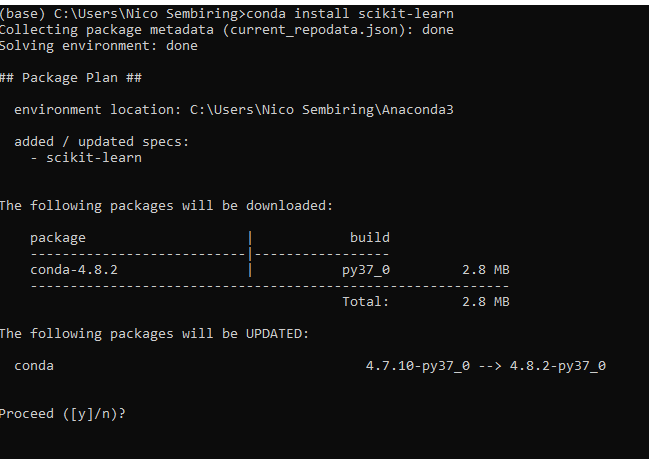
\includegraphics[width=4cm]{figures/1174096/1/install1.PNG}
            \centering
            \caption{Instalasi Package Scikit Learn}
        \end{figure}
		\hfill\break
		Klasifikasi adalah pengelompokan data di mana data yang digunakan memiliki label atau kelas target. Sehingga algoritma untuk menyelesaikan masalah klasifikasi dikategorikan ke dalam pembelajaran terbimbing.
		\item Kemudian pilih Y
		\begin{figure}[H]
            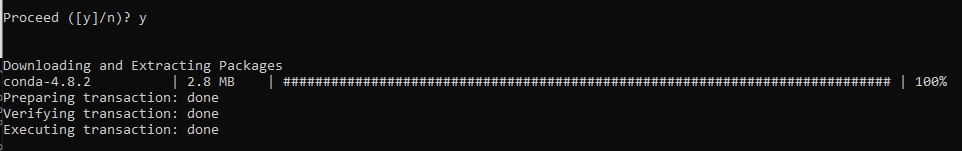
\includegraphics[width=4cm]{figures/1174096/1/install2.PNG}
            \centering
            \caption{pilih y}
        \end{figure}
	\end{itemize}
	
	\item Mencoba loading an example dataset
	\hfill\break
	\lstinputlisting[firstline=8, lastline=12]{src/1174096/1/1174096.py}
	\item Mencoba Learning dan predicting
	\hfill\break
	\lstinputlisting[firstline=14, lastline=24]{src/1174096/1/1174096.py}
	\item Mencoba Model Persistence
	\hfill\break
	\lstinputlisting[firstline=26, lastline=36]{src/1174096/1/1174096.py}
	\item Mencoba Conventions
	\hfill\break
	\lstinputlisting[firstline=38, lastline=56]{src/1174096/1/1174096.py}
\end{enumerate}
\subsection{Penanganan Error}
\begin{enumerate}
	\item ScreenShoot Error
	\begin{figure}[H]
		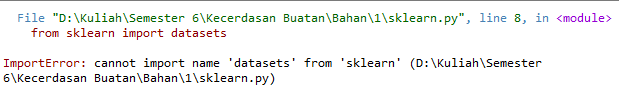
\includegraphics[width=4cm]{figures/1174096/error/1_import.png}
		\centering
		\caption{Import Error}
	\end{figure}
	\begin{figure}[H]
		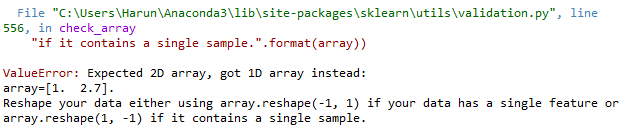
\includegraphics[width=4cm]{figures/1174096/error/1_value.png}
		\centering
		\caption{Value Error}
	\end{figure}
	\item Tuliskan Kode Error dan Jenis Error
	\begin{itemize}
		\item Import Error
		\item Value Error
	\end{itemize}
	\item Cara Penangan Error
	\begin{itemize}
		\item Import Error
		\hfill\break
		Dengan Menginstall Library Yang Tidak Ditemukan
		\item Value Error
		\hfill\break
		Mengubah Bentuk Arraynya, Menjadi 1 Dimensi
	\end{itemize}
\end{enumerate}
\subsection{Bukti Tidak Plagiat}
\begin{figure}[H]
	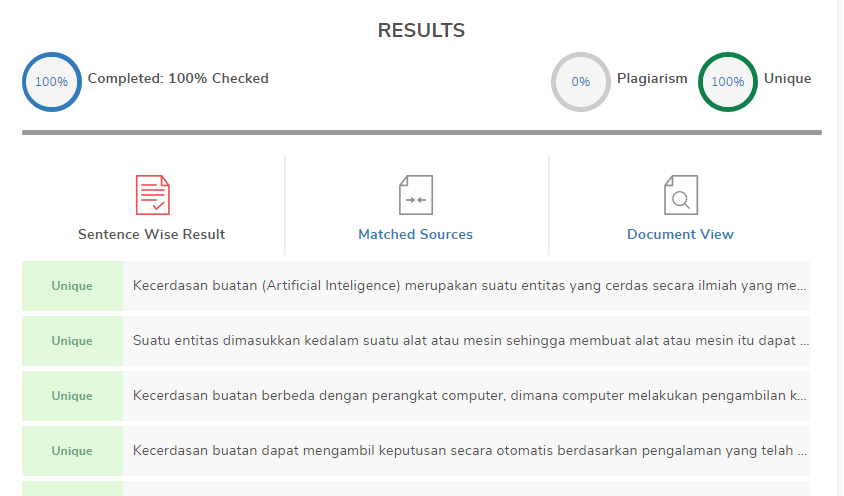
\includegraphics[width=4cm]{figures/1174096/bukti/plagiarisme.PNG}
	\centering
	\caption{Bukti Tidak Plagiarisme}
\end{figure}